%%%%%%%%%%%%%%%%%%%%%%%%%%%%%%%%%%%%%%%%%%%%%%%%%%%%%%%%%%%%%%%%%%%%%%
% Lớp 10 | Bất phương trình bậc 2 một ẩn | Giải bất phương trình bậc 2 một ẩn
% Dạng 0D7?2-2: Giải bất phương trình bậc hai biết BXD, đồ thị
% Số câu: 10  (sinh tự động bởi tach_cau.py; từ nay thầy sửa trực tiếp file này)
%%%%%%%%%%%%%%%%%%%%%%%%%%%%%%%%%%%%%%%%%%%%%%%%%%%%%%%%%%%%%%%%%%%%%%

%%%%%%%%%%%%%%%% TRẮC NGHIỆM 4 PHƯƠNG ÁN %%%%%%%%%%%%%%%%

% nguồn: MaHoaNH_TracNghiem_Lop10
\begin{ex}%[0D7N2-2]%[ma:344abdff]
	Bất phương trình  $9x^2+1\leq 6x$ có tập nghiệm là
	 \choice
		 {$\left\{-\dfrac{1}{3}\right\}$}
		{\True $\left\{\dfrac{1}{3}\right\}$} 
		{$\varnothing$} 
		{$\mathbb{R}$} 
	 \loigiai{
		Ta có  $9x^2+1\leq6x\Leftrightarrow9x^2-6x+1\leq0\Leftrightarrow(3x-1)^2\le0\Leftrightarrow x=\dfrac{1}{3}$.\\
		Vậy tập  nghiệm của bất phương trình là $S=\left\{\dfrac{1}{3}\right\}$.
	 }
\end{ex}

% nguồn: MaHoaNH_TracNghiem_Lop10
\begin{ex}%[0D7N2-2]%[ma:299937c7]
	Cho đồ thị của hàm số bậc hai $f(x)$ như  hình vẽ
	\begin{center}
		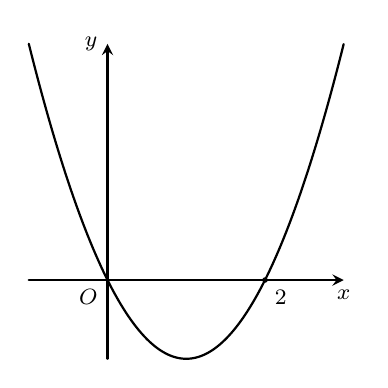
\begin{tikzpicture}[scale=1,font=\footnotesize,line join=round,line cap=round,>=stealth]
				 \draw[thick,->] (-1,0)--(3,0) node[below] {$x$};
				\draw[thick,->] (0,-1)--(0,3) node[left]  {$y$};
				\draw (0,0)  node[below left] {$O$};
				\draw[thick,smooth,samples=200] plot[domain=-1:3] (\x,{(\x)^2-2*(\x)}); 
				\fill  (2,0) circle (1pt) node[below right] {$2$};
			\end{tikzpicture}
	\end{center}
	Tập nghiệm của bất phương trình  $f(x)>0$ là
	 \choice
		{\True $S=(-\infty; 0) \cup  (2;+\infty)$}
		{$S=(0;  2)$}
		{$S=(-\infty; 0]  \cup [2;+\infty)$}
		{$S=(2;+\infty)$} 
	\loigiai{ 
		Dựa vào đồ thị hàm số bậc hai $f(x)$ đã cho, ta thấy phần đồ  thị nằm phía trên trục hoành khi $x<0$ hoặc $x>2$.\\
		Vậy tập nghiệm của bất phương trình $f(x)>0$ là $S=(-\infty; 0) \cup  (2;+\infty)$.
	} 
\end{ex}

% nguồn: MaHoaNH_TracNghiem_Lop10
\begin{ex}%[0D7H2-2]%[ma:1636c801]
	Tập nghiệm của  bất phương trình $x^2-7x+12<0$ là
	 \choice
		 {$\varnothing$}
		 {$(-\infty;3) \cup (4;+\infty)$}
		{\True  $(3;4)$}
		 {$(0;4)$}
	 \loigiai{
		 Xét phương trình $x^2-7x+12=0 \Leftrightarrow x=3$ hay $x=4$.
		\begin{center}
			\begin{tikzpicture}[smooth,samples=300,scale=0.5,>=stealth,font=\footnotesize]
					\tkzTabInit[lgt=4.5] 
						 {$x$/1,$x^2-7x+12$/1}
						{$-\infty$,$3$,$4$,$+\infty$} 
					\tkzTabLine{,+,0,-,0,+,} 
				\end{tikzpicture}
		\end{center}
		 Tập nghiệm của bất phương trình $x^2-7x+12<0$ là $(3;4)$.
	 }
\end{ex}

% nguồn: MaHoaNH_TracNghiem_Lop10
\begin{ex}%[0D7H2-2]%[ma:db0d1e61]
	Cho tam thức bậc hai $f(x)=-x^2-4x+5$. Tìm tất cả  giá trị của $x$ để $f(x)\ge 0$.
	 \choice
		{$x\in \left(-\infty;-1\right]\cup \left[5;+\infty \right)$} 
		{$x\in \left[-1; 5\right]$} 
		{\True  $x\in \left[-5; 1\right]$}
		{$x\in \left(-5; 1\right)$} 
	 \loigiai{
		Xét tam  thức $f(x)=-x^2-4x+5$. Ta có
		\begin{itemize}
			\item $a=-1<  0$;
			\item $\Delta=36> 0$ nên tam thức $f(x)$ có hai nghiệm $x=1$ và $x=-5$. 
		\end{itemize}
		Bảng xét dấu 
		\begin{center}
			\begin{tikzpicture}[>=stealth]
					\tkzTabInit[nocadre=false,lgt=1.5,espcl=2,deltacl=0.6]{$x$/.7,$f  (x)$/.7}
						{$-\infty$,$-5$,$1$,$+\infty$} 
					\tkzTabLine{,-,$0$,+,$0$,-,} 
				\end{tikzpicture}
		\end{center}
		Suy ra $f(x)\ge 0$ khi $-5\le x\le  1$.
	 }
\end{ex}

% nguồn: MaHoaNH_TracNghiem_Lop10
\begin{ex}%[0D7H2-2]%[ma:1d443a21]
	Bảng xét dấu  nào sau đây là bảng xét dấu của tam thức $f(x)=-x^2-x+6$?
	 \choice
		{\begin{tikzpicture}
		\tkzTabInit[nocadre=false,lgt=1.5,espcl=1.5] 
			{$x$ /0.6,$f  (x)$ /0.6}
			{$-\infty$,$-2$,$3$,$+\infty$} 
		\tkzTabLine{,-,0,+,0,-} 
	\end{tikzpicture}
		 }
		{\begin{tikzpicture}
		\tkzTabInit[nocadre=false,lgt=1.5,espcl=1.5] 
			 {$x$ /0.6,$f (x)$ /0.6}
			{$-\infty$,$-2$,$3$,$+\infty$} 
		 \tkzTabLine{,+,0,-,0,+}
	\end{tikzpicture}
		} 
		{\True \begin{tikzpicture}
		\tkzTabInit[nocadre=false,lgt=1.5,espcl=1.5] 
			 {$x$ /0.6,$f (x)$ /0.6}
			{$-\infty$,$-3$,$2$,$+\infty$} 
		\tkzTabLine{,-,0,+,0,-} 
	\end{tikzpicture}
		 }
		{\begin{tikzpicture}
		 \tkzTabInit[nocadre=false,lgt=1.5,espcl=1.5]
			{$x$  /0.6,$f (x)$ /0.6}
			{$-\infty$,$-3$,$2$,$+\infty$} 
		 \tkzTabLine{,+,0,-,0,+}
	\end{tikzpicture}
		 }
	\loigiai{ 
		Tam thức $f(x)=-x^2-x+6$ có $\Delta =25>0$, hai nghiệm $x_1=-3$, $x_2=2$  và hệ số $a=-1<0$.\\
		Suy ra bảng xét dấu của $f(x)$  như sau
		\begin{center}
			\begin{tikzpicture}
					 \tkzTabInit[nocadre=false,lgt=1.5,espcl=1.5]
						{$x$ /0.6,$f (x)$ /0.6} 
						{$-\infty$,$-3$,$2$,$+\infty$} 
					 \tkzTabLine{,-,0,+,0,-}
				\end{tikzpicture}
		\end{center}
	} 
\end{ex}


%%%%%%%%%%%%%%%% ĐÚNG/SAI %%%%%%%%%%%%%%%%

% nguồn: MaHoaNH_DungSai_Lop10
\begin{ex}%[0D7H2-2]%[ma:f645a8c3]
	\immini{Cho hàm số $f(x)=ax^2+bx+c$  có đồ thị như hình bên.
	\choiceTF 
		 {Hàm số đồng biến trên $(1;3)$}
		{Phương  trình $f(x)=0$ vô nghiệm}
		{\True Trục đối xứng của đồ thị hàm số có  phương trình $x=2$}
		{\True $f(x)<0\Leftrightarrow  x \in (1;3)$}
		 }{
		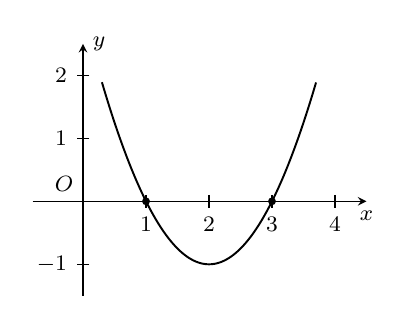
\begin{tikzpicture}[smooth,samples=300,scale=0.8,>=stealth,font=\footnotesize]
				 \draw[->] (-0.8,0)--(4.5,0) node[below]{$x$};
				\draw[->] (0,-1.5)--(0,2.5) node[right]{$y$}; 
				 \draw (0,0) node[above left]{$O$};
				\draw[line  width=0.7pt,domain=0.3:3.7] plot (\x,{(\x)^2-4*(\x)+3});
				\draw[fill=black] (1,0) circle (1.5pt) 
					(3,0)  circle (1.5pt);
				\foreach \x  in {1,2,3,4}\draw (\x,0.1)--(\x,-0.1) node [below] {\footnotesize $\x$};
				\foreach \y in {-1,1,2}\draw (0.1,\y)--(-0.1,\y) node [left]  {\footnotesize $\y$};
			\end{tikzpicture}
		 }
	 \loigiai{
		\begin{itemchoice}
			\itemch Sai. Vì hàm số  đồng biến trên các khoảng $(-\infty;1)$ và $(3;+\infty)$.
			\itemch Sai. Vì phương trình có hai nghiệm  $x=1$ hoặc $x=3$.
			\itemch Đúng. Vì trục đối xứng của đồ thị hàm số có  phương trình $x=2$.
			\itemch Đúng. Vì $f(x)<0$  thì $1<x<3$.
		\end{itemchoice}
	 }
\end{ex}

% nguồn: MaHoaNH_DungSai_Lop10
\begin{ex}%[0D7H2-2]%[ma:02870b30]
	 \immini
	 {
	Cho hàm số bậc hai $f(x)=ax^2+bx+c$ có đồ thị  như hình vẽ bên.
	\choiceTF 
		{\True  $a>0$}
		 {$f(0)=1$}
		{Phương trình $f(x)=0$ có hai  nghiệm trái dấu}
		{\True Tập nghiệm của bất  phương trình là $f(x)>0$ là $(-\infty;1)\cup(2;+\infty)$}
		 }
		{ 
		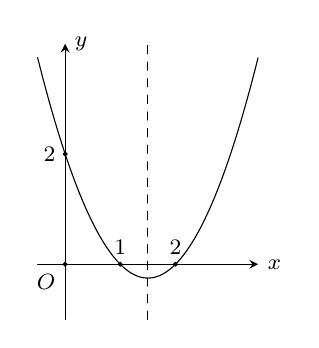
\begin{tikzpicture}[line cap=round,line join=round,>=stealth,font=\footnotesize,scale=0.7]
				\def\xmin{-.5} 
				\def\xmax{3.5} 
				 \def\ymin{-1}
				\def\ymax{4} 
				\draw[-stealth] (\xmin,0)--(\xmax,0)  node[right]{$x$};
				 \draw[-stealth] (0,\ymin)--(0,\ymax) node[right]{$y$};
				 \draw[samples=200,domain=\xmin:\xmax]plot (\x,{(\x)^2-3*(\x)+2});
				\draw[fill=black] (0,0) circle (1pt) node[below  left]{$O$};
				\draw[dashed]  (1.5,\ymin)--(1.5,\ymax);
				\clip (\xmin,\ymin)  rectangle (\xmax,\ymax);
				 \fill[draw] (1,0) node[above]{$1$} circle (1pt);
				\fill[draw]  (2,0) node[above]{$2$} circle (1pt);
				\fill[draw] (0,2)  node[left]{$2$} circle (1pt);
			\end{tikzpicture}
		} 
	\loigiai{ 
		\begin{itemchoice}
			 \itemch Từ đồ thị hàm số $f(x)$ ta thấy bề lõm hướng lên nên suy ra $a>0$.
			\itemch Từ  đồ thị hàm số $f(x)$ ta có $f(0)=2$.
			\itemch Từ đồ thị hàm số $f(x)$  ta có $f(x)=0 \Leftrightarrow \hoac{&x=1>0\\&x=2>0.}$
			\itemch Từ đồ thị hàm số $f(x)$ ta có  bảng xét dấu
			\begin{center}
				\begin{tikzpicture}
					 \tkzTabInit[lgt=1.2,espcl=2.5,deltacl=0.6]
						 {$x$/0.6,$f (x)$/0.6}{$-\infty$,$1$,$2$,$+\infty$}
					\tkzTabLine{,+,0,-,0,+,} 
				\end{tikzpicture}
			\end{center}
			Tập nghiệm của bất phương trình $f(x)>0$  là $S=(-\infty;1)\cup(2;+\infty)$.
		\end{itemchoice}
	} 
\end{ex}

% nguồn: MaHoaNH_DungSai_Lop10
\begin{ex}%[0D7H2-2]%[ma:59354ede]
	Các  mệnh đề sau đúng hay sai?
	\choiceTF 
		{$7x^2-4x-3< 0\Leftrightarrow x\in \left(-\infty;-\dfrac{3}{7}  \right)\cup \left(1;+\infty \right)$}
		 {$-x^2+6x-9\ge 0\Leftrightarrow x\in \mathbb{R}$}
		{\True $-5x^2+4x+12< 0\Leftrightarrow x\in \left(-\infty;-\dfrac{6}{5}  \right)\cup (2;+\infty)$}
		{\True $3x^2-4x+4\ge  0\Leftrightarrow x\in \mathbb{R}$}
	 \loigiai{
		\begin{itemchoice}
			\itemch Sai. $7x^2-4x-3=0\Leftrightarrow x=1$ hoặc  $x=-\dfrac{3}{7}$.\\
			 Bảng xét dấu
			\begin{center}
				\begin{tikzpicture}[>=stealth]
						\tkzTabInit[nocadre=false,lgt=1.5,espcl=2,deltacl=0.6]{$x$/.7,$f (x)$/.7} 
						 {$-\infty$,$-\tfrac{3}{7}$,$1$,$+\infty$}
						\tkzTabLine{,+,$0$,-,$0$,+,} 
					\end{tikzpicture}
			\end{center}
			Ta  có $7x^2-4x-3< 0\Leftrightarrow x\in \left(-\dfrac{3}{7};1\right)$.\\
			Vậy tập nghiệm  bất phương trình là $S=\left(-\dfrac{3}{7};1\right)$.
			\itemch Sai. $-x^2+6x-9=0\Leftrightarrow x=3$.\\ 
			Bảng xét  dấu
			\begin{center}
				\begin{tikzpicture}[>=stealth]
						\tkzTabInit[nocadre=false,lgt=1.5,espcl=2,deltacl=0.6]{$x$/.7,$f (x)$/.7} 
						 {$-\infty$,$3$,$+\infty$}
						\tkzTabLine{,-,$0$,-,} 
					\end{tikzpicture}
			\end{center}
			Ta có $-x^2+6x-9\ge 0\Leftrightarrow  x\in \{3\}$.
			 Vậy tập nghiệm bất phương trình là $S=\{3\}$.
			\itemch Đúng. $-5x^2+4x+12=0\Leftrightarrow x=2$  hoặc $x=-\dfrac{6}{5}$.\\
			 Bảng xét dấu
			\begin{center}
				\begin{tikzpicture}[>=stealth]
						\tkzTabInit[nocadre=false,lgt=1.5,espcl=2,deltacl=0.6]{$x$/.7,$f (x)$/.7} 
						{$-\infty$,$-\tfrac{6}{5}$,$2$,$+\infty$} 
						\tkzTabLine{,-,$0$,+,$0$,-,} 
					\end{tikzpicture}
			\end{center}
			Ta có $-5x^2+4x+12<  0\Leftrightarrow x\in \left(-\infty;-\dfrac{6}{5} \right)\cup (2;+\infty)$.\\
			Vậy tập nghiệm bất  phương trình là: $S=\left(-\infty;-\dfrac{6}{5} \right)\cup (2;+\infty)$.
			\itemch Đúng. Tam thức $3x^2-4x+4$ có $\heva{&a=3>0\\&\Delta'=-8<0}\Rightarrow 3x^2-4x+4\geq  0,\,\forall x\in\mathbb{R}$.
		\end{itemchoice}
	 }
\end{ex}


%%%%%%%%%%%%%%%% TỰ LUẬN %%%%%%%%%%%%%%%%

% nguồn: MaHoaNH_TuLuan_Lop10
\begin{bt}%[0D7B2-2]%[ma:cb24c0c5]
	 Giải bất phương trình $(x^2-3x+2)(x^2-1)\le 0$.
	\loigiai{ 
		Ta  có
		 \allowdisplaybreaks
		$\begin{aligned}
		 &\quad (x^2-3x+2)(x^2-1)\le 0 \Leftrightarrow (x-1)^{2}(x+1)(x-2)\le 0\\
		&\Leftrightarrow \hoac{&x-1=0\\&(x+1)(x-2)\le 0} \Leftrightarrow \hoac{&x=1\\&-1\le  x\le 2.}
	\end{aligned}$\\
	Vậy bất phương  trình có tập nghiệm $S=[-1;2]$.
} 
\end{bt}

% nguồn: MaHoaNH_TuLuan_Lop10
\begin{bt}%[0D7B2-2]%[ma:59b9d41e]
	Giải bất phương trình sau $(x^2+5x)(1-x^2)\ge  0$.
	\loigiai{ 
		Ta có $x^2+5x=0\Leftrightarrow\hoac{&x=-5\\&x=0}$. Lại có $1-x^2=0\Leftrightarrow x=\pm  1$.\\
		Bảng xét dấu vế trái  của bất phương trình
		\begin{center}
			\begin{tikzpicture}
					\tkzTabInit[nocadre=false,lgt=4,espcl=2,deltacl=0.5] 
						{$x$/1,$x^2+5x$/1,$1-x^2$/1,$(x^2+5x) 
						 (1-x^2)$/1}
						{$-\infty$,$-5$,$-1$,$0$,$1$,$+\infty$} 
					 \tkzTabLine{,+,z,-,t,-,z,+,t,+}
					 \tkzTabLine{,-,t,-,z,+,t,+,z,-}
					 \tkzTabLine{,-,z,+,z,-,z,+,z,-}
				\end{tikzpicture}
		\end{center}
		Dựa vào bảng xét dấu, suy ra bất phương trình có tập nghiệm  $S=[-5;-1]\cup[0;1]$.
	 }
\end{bt}
